\subsection*{Problema 12}

\textbf{Enunciado:} 
Calcular la integral:
\begin{align*}
\int \dfrac{x^4}{x^4 - 1} \, dx
\end{align*}

\textbf{Solución:} 
Dado que el grado del numerador es igual al grado del denominador, realizamos la división polinómica:
\begin{align*}
\dfrac{x^4}{x^4 - 1} = 1 + \dfrac{1}{x^4 - 1}
\end{align*}

Factorizamos el denominador como se indica en las observaciones:
\begin{align*}
x^4 - 1 = (x - 1)(x + 1)(x^2 + 1)
\end{align*}

Planteamos la descomposición en fracciones parciales para la fracción restante:
\begin{align*}
\dfrac{1}{x^4 - 1} &= \dfrac{A}{x - 1} + \dfrac{B}{x + 1} \\
&+ \dfrac{Cx + D}{x^2 + 1}
\end{align*}

Multiplicando por el denominador común y evaluando para hallar los coeficientes, obtenemos:
\begin{align*}
A &= \dfrac{1}{4}, \quad B = -\dfrac{1}{4}, \quad C = 0, \quad D = -\dfrac{1}{2}
\end{align*}

Sustituyendo los valores, la integral se reescribe como:
\begin{align*}
\int &\left( 1 + \dfrac{1/4}{x - 1} - \dfrac{1/4}{x + 1} - \dfrac{1/2}{x^2 + 1} \right) dx
\end{align*}

Integramos cada término por separado:
\begin{align*}
\int 1 \, dx &= x \\
\int \dfrac{1/4}{x - 1} \, dx &= \dfrac{1}{4} \ln|x - 1| \\
\int -\dfrac{1/4}{x + 1} \, dx &= -\dfrac{1}{4} \ln|x + 1| \\
\int -\dfrac{1/2}{x^2 + 1} \, dx &= -\dfrac{1}{2} \arctan(x)
\end{align*}

Juntando todos los resultados y añadiendo la constante de integración $C$, obtenemos la solución general:
\begin{align*}
F(x) &= x + \dfrac{1}{4} \ln\left|\dfrac{x - 1}{x + 1}\right| \\
&- \dfrac{1}{2} \arctan(x) + C
\end{align*}

\begin{figure}[H]
	\centering
	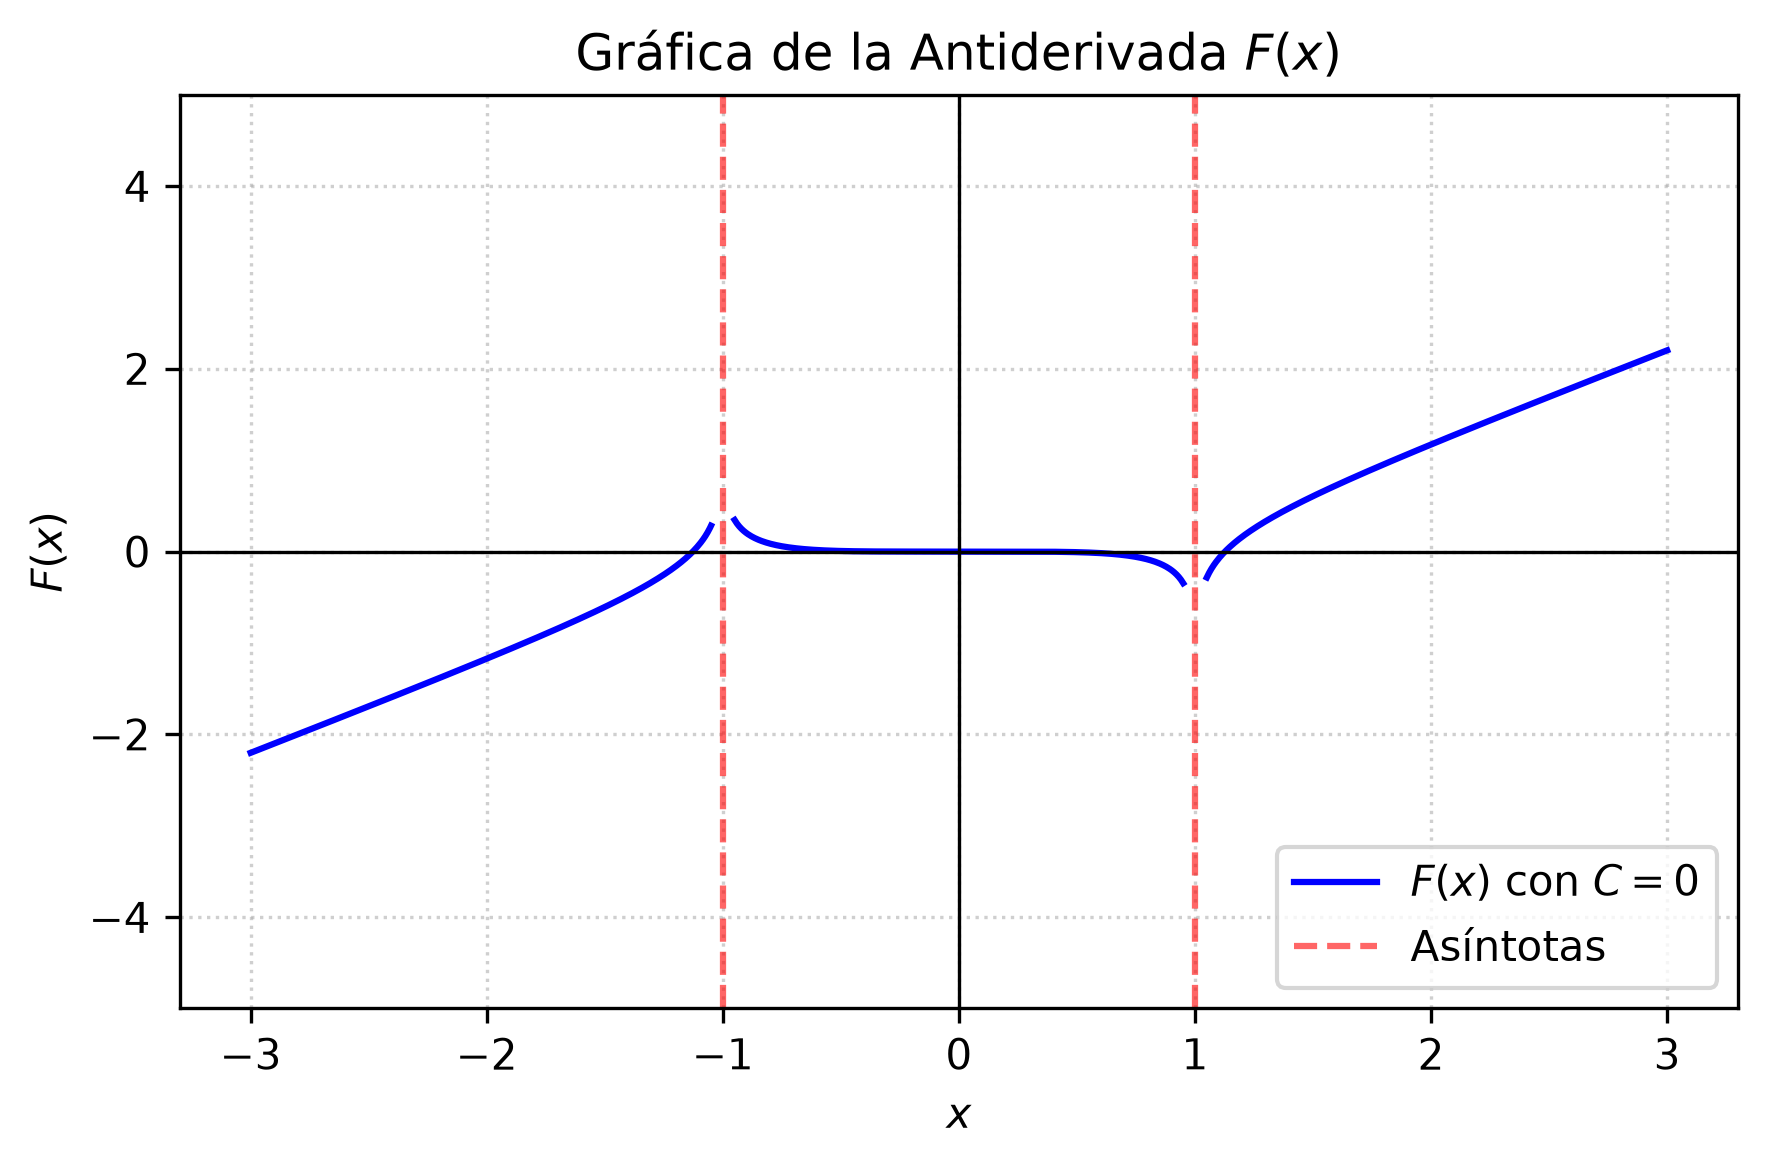
\includegraphics[width=\columnwidth]{semana_03/graficas/SEM03_P12_grafica.png}
	\caption{Representación gráfica de $f(x)$ y su antiderivada $F(x)$ evaluada para la constante de integración $C = 0$ (Problema 12).}
	\label{fig:problema12}
\end{figure}
